\paragraph{В четвертой} главе приводится полунатурный эксперимент по проверке рабочих характеристик предложенного комплексированного алгоритма
оценки информационных параметров CDMA-сигнала на фоне аддитивного белого гауссового шума и интерференционной помехи.
Эксперимент проводился на оригинальной, разработанной автором, программно-аппаратной платформе.
В качестве микросхемы захвата сигнала использовался чип от компании Maxim Semiconductor - MAX2769. Длинна записи, получаемой
с данной платформы для постобработки составляет 32 мс. Этого объема данных хватает для проверки качества работы алгоритма при оценке
параметров сигнала, но к сожалению не хватает для запуска модуля фазовой автоподстройки частоты для проверки вхождения в синхронизм и точной оценки частоты.

В данном случае, так как точное значение на выходе ФАПЧ получить не удается, за точное значение частоты бралось среднее значение математических
ожиданий всех оценок типового и комплексированного алгоритмов. Результаты эксперимента представлены в таблице \ref{tbl:16MHz}.

{\centering
\begin{longtable}{ | c | c | c |}
	%\captionsetup{justification=raggedleft,singlelinecheck=off}
	\caption{}\label{tbl:16MHz} \\
	\hline
	Алгоритм	& Вероятность	& Дисперсия, Гц \\
			& правильной оценки&		\\ \hline
	АР + DMA	& 0.52 & 16.13	\\ \hline
	Коррелятор 	& 0.80 &  21.56 \\ \hline
\end{longtable}}

Так же в данной главе приводится полунатурное моделирование на данных, полученных из внешних источников. Длинна записи данных
позволяет оценить как параметры параметры сигнала, так и запустить модуль фазовой автоподстройки частоты для проверки вхождения в синхзронизм.

Результаты полунатурного эксперимента на данных, полученных из внешних источников, представлены в таблице \ref{tbl:5MHz}.
Эксперимент показал, что предлагаемый подход позволяет получить более точную оценку параметров
сигнала в системе с кодовым разделением каналов на примере системы Navstar GPS, а так же войти в синхронизм.

{\centering
\begin{longtable}{ | c | c | c | c |}
	%\captionsetup{justification=raggedleft,singlelinecheck=off}
	\caption{}\label{tbl:5MHz} \\
	\hline
	Алгоритм	& Вероятность	& Дисперсия, Гц & Среднее время \\
			& правильной оценки&		& вхождения в синхронизм\\ \hline
	АР + DMA	& 0.57 		& 15.42		& 21 мс \\ \hline
	Коррелятор 	& 0.84 		& 23.15 	& 34 мс \\ \hline
\end{longtable}}

Результаты данных полунатурных экспериментов показали, что предлагаемый подход позволяет получить более точную оценку параметров
сигнала в CDMA-системе на примере системы Navstar GPS.

%\paragraph{В четвертой} главе приводится имитационное моделирование развиваемых алгоритмов. В качестве алгоритма
%для сравнения используется параллельный коррелятор с алгоритмом уточнения частоты.
%
%\noindent{\begin{figure}[H]
%\center\scalebox{0.65}{\includegraphics[width=1\linewidth]{modeling_general.eps}}
%	\caption{Схема эксперимента}
%	%\label{pic:ar_dma_probability}
%\end{figure}}
%
%\underline{Алгоритм} оценки параметров сигнала с расширенным спектром на фоне аддитивного белого шума.
%График вероятности оценки частоты в допустимом диапазоне входной расстройки представлен на рисунке
%\ref{pic:lpc_for_1_probability}. Моделирование проводилось с аддитивным шумом, заданным в полосе от 0 Гц до
%половины частоты дискретизации для одного, двух и трех шагов уточнения АКФ. В данном случае значение частоты дискретизации равно 16.368 МГц.
%\begin{figure}[H]
%\center\scalebox{1}{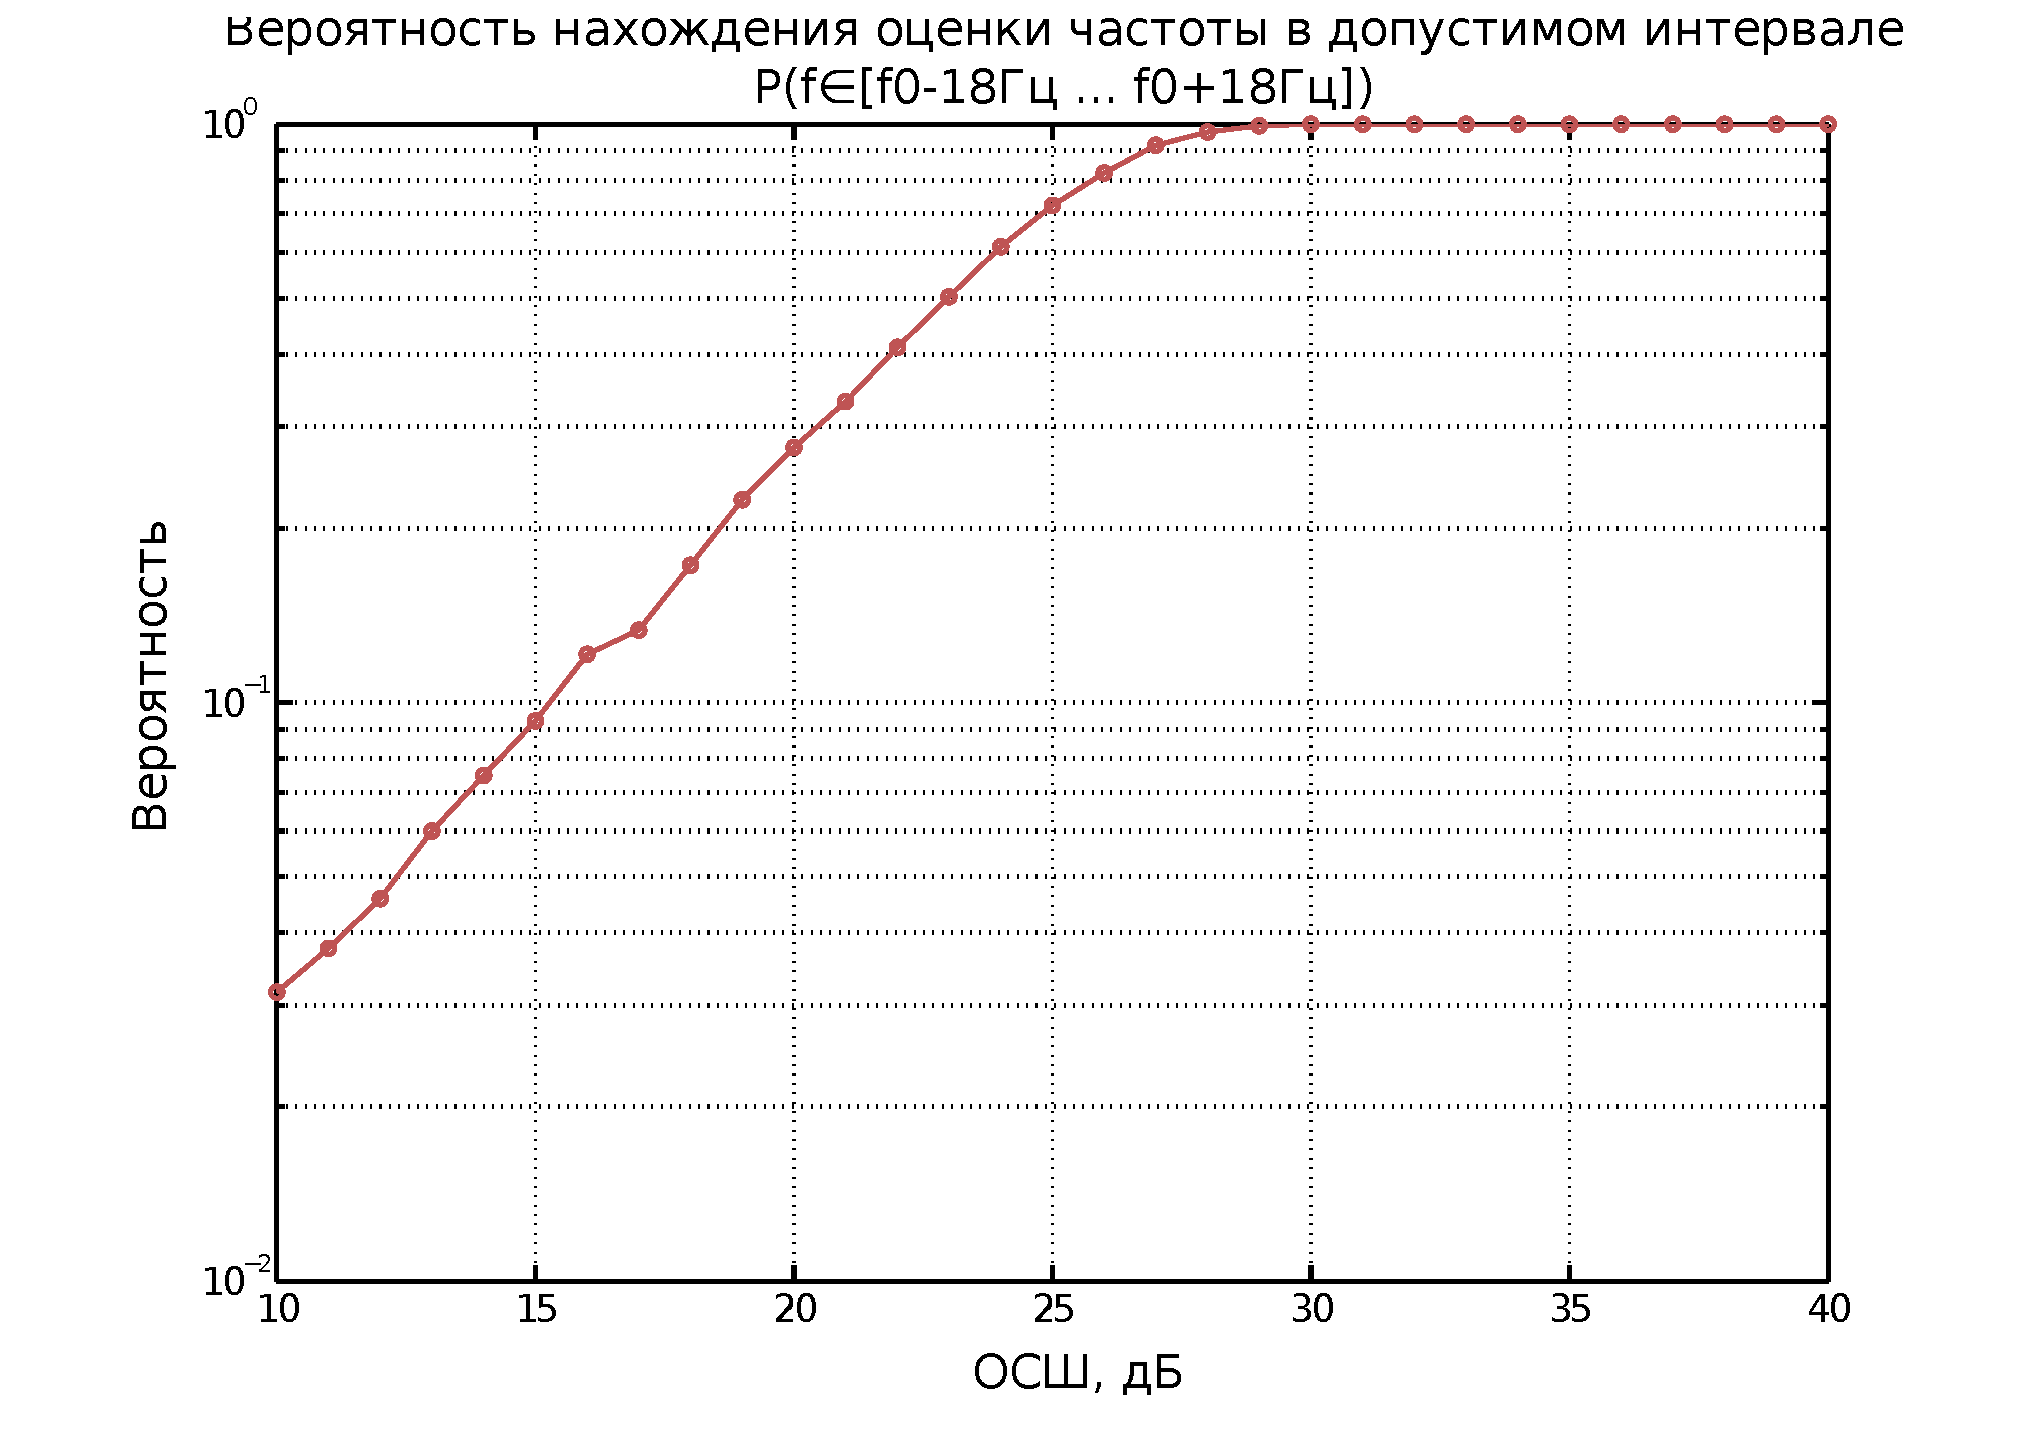
\includegraphics[width=1\linewidth]{lpc_for_1_probability.eps}}
%	\caption{Вероятность оценки частоты удовлетворяющей допустимой входной расстройке}
%	\label{pic:lpc_for_1_probability}
%\end{figure}
%
%Для оценки точности можно сравнить предлагаемый алгоритм с границей Крамера-Рао. Неравенство Крамера-Рао дает базу оценки, так
%как представляет минимальную дисперсию среди всех классов оценщиков.
%\begin{figure}[H]
%\center\scalebox{1}{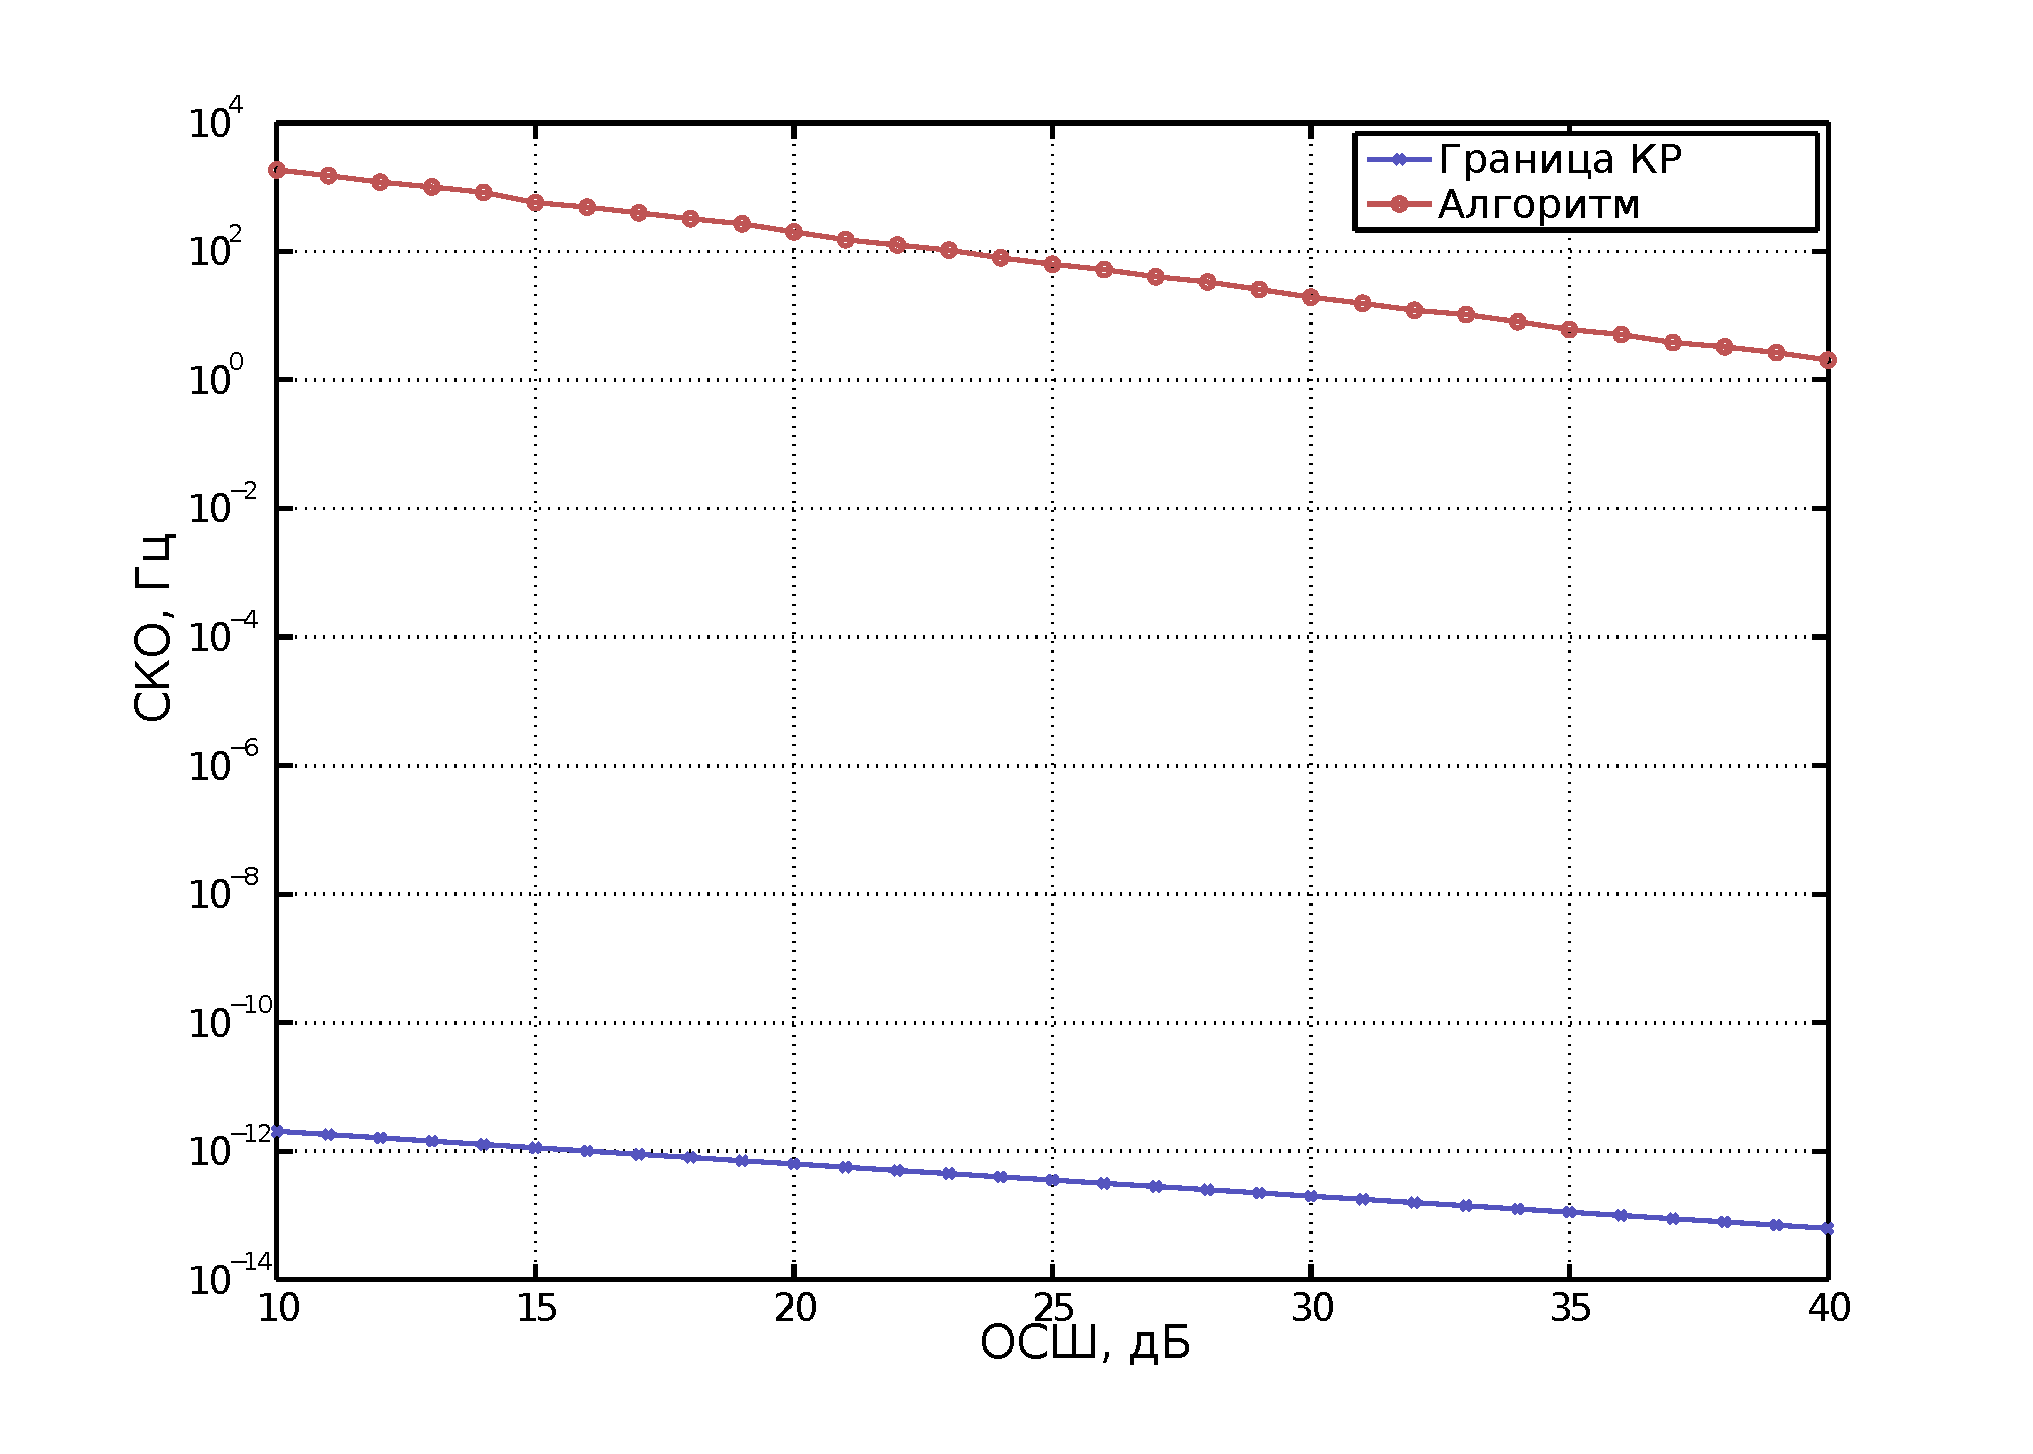
\includegraphics[width=1\linewidth]{crlb_vs_1sat_algo.eps}}
%	\caption{СКО ошибка оценки частоты и граница Крамера-Рао в задаче оценки частоты гармонического сигнала}
%	\label{pic:crlb_vs_1sat_algo}
%\end{figure}
%
%%%%%%%%%%
%\underline{Алгоритм} оценки параметров ШПС в условиях интерференции и аддитивного белого шума
%(Delay and Multiply Approach + уточненный АР).
%
%График вероятности оценки частоты в допустимом диапазоне входной расстройки представлен на рисунке
%\ref{pic:ar_dma_probability}. Моделирование проводилось с аддитивным шумом, заданным в полосе от 0 Гц до
%половины частоты дискретизации для одного, двух и трех шагов уточнения АКФ. В данной имитационной модели значение частоты дискретизации равно 16.368 МГц.
%\begin{figure}[H]
%\center\scalebox{1}{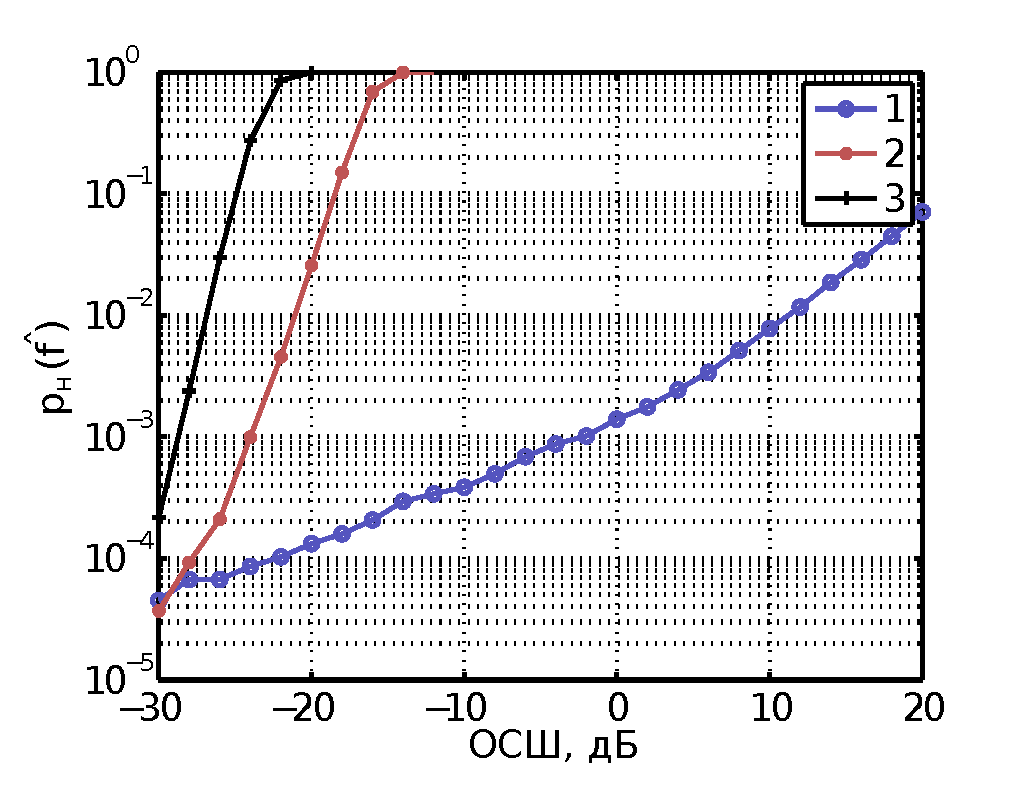
\includegraphics[width=1\linewidth]{ar_dma_probability.eps}}
%	\caption{Вероятность оценки частоты удовлетворяющей допустимой входной расстройке}
%	\label{pic:ar_dma_probability}
%\end{figure}
%
%Так же интересным является сравнение качество оценки частоты. График СКО ошибки при оценке частоты в зависимости
%от ОСШ представлен на рисунке \ref{pic:crlb_vs_snr}. Для сравнения так же взята граница Крамера-Рао (КР).
%\begin{figure}[H]
%\center\scalebox{1}{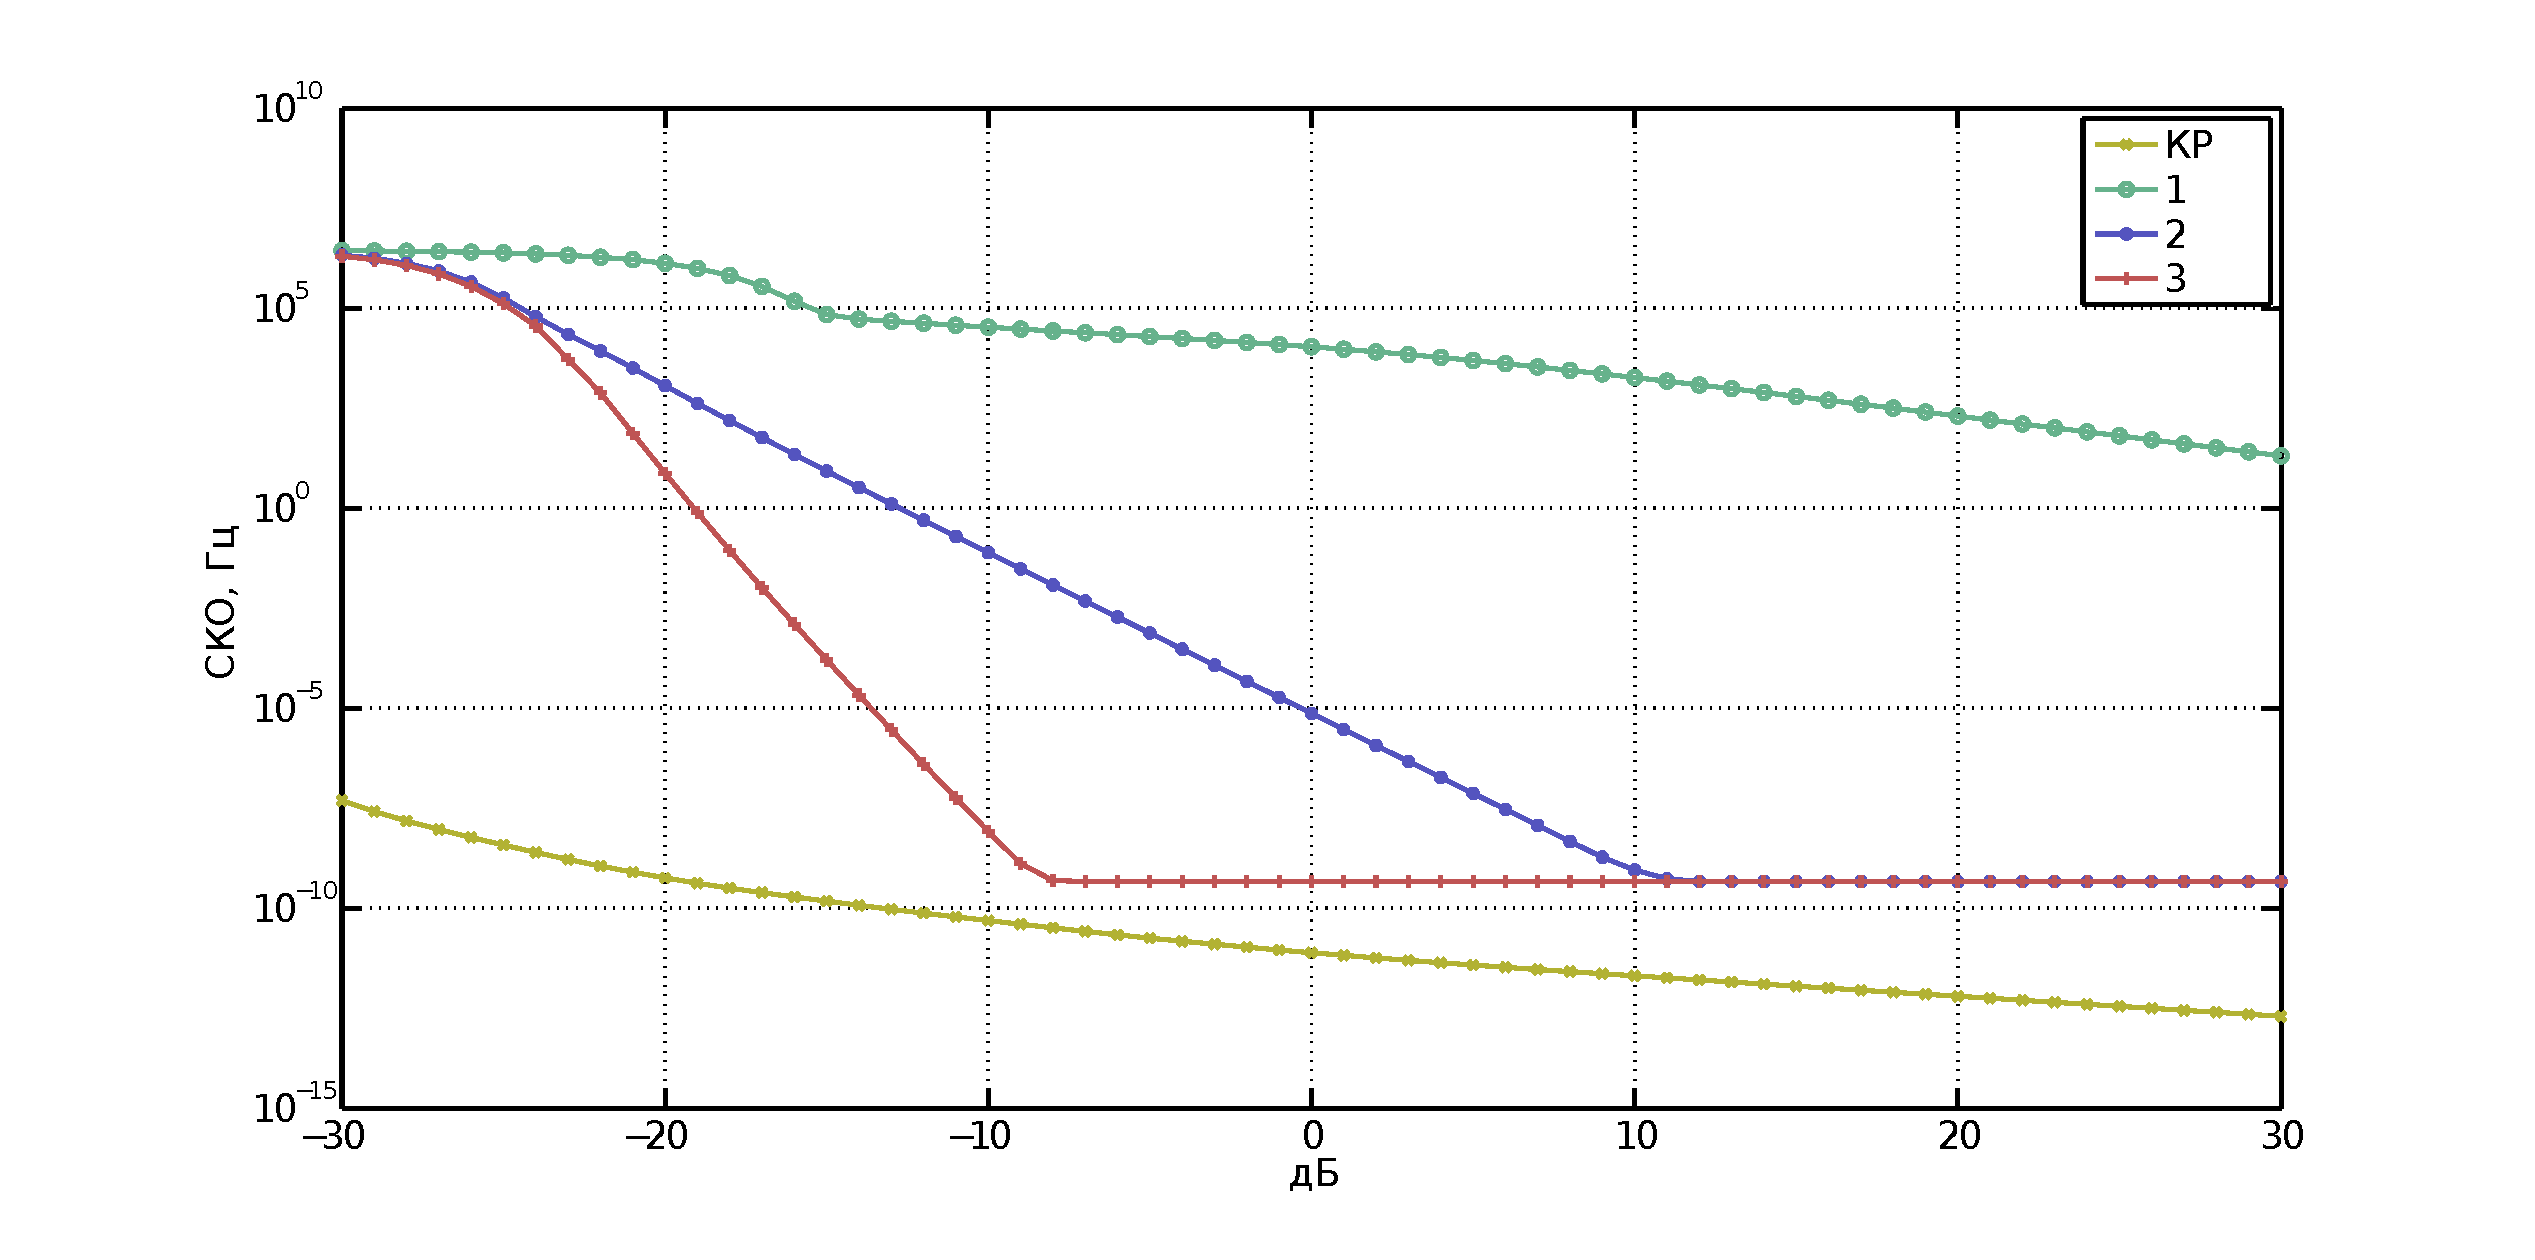
\includegraphics[width=1\linewidth]{crlb_vs_snr.eps}}
%	\caption{СКО ошибка оценки частоты и граница Крамера-Рао в задаче оценки частоты гармонического сигнала}
%	\label{pic:crlb_vs_snr}
%\end{figure}
